\section{Chapter 2}
\colorbox{black}{\textbf{\color{white}Definitions}}
\begin{itemize}
    \item $v_i$ is {\color{red}adjacent} to $v_j$, or symbolically as $v_i \sim v_j$, if an edge exists between $v_i$ and $v_j$, or symbolically as $v_i v_j \in E$. Edge $v_i v_j$ is {\color{red}incident} with vertices $v_i$ and $v_j$.
    \item Example of an undirected, unweighted graph, $\mathcal{G}=(V,E)$
    \begin{figure}[H]
        \centering
        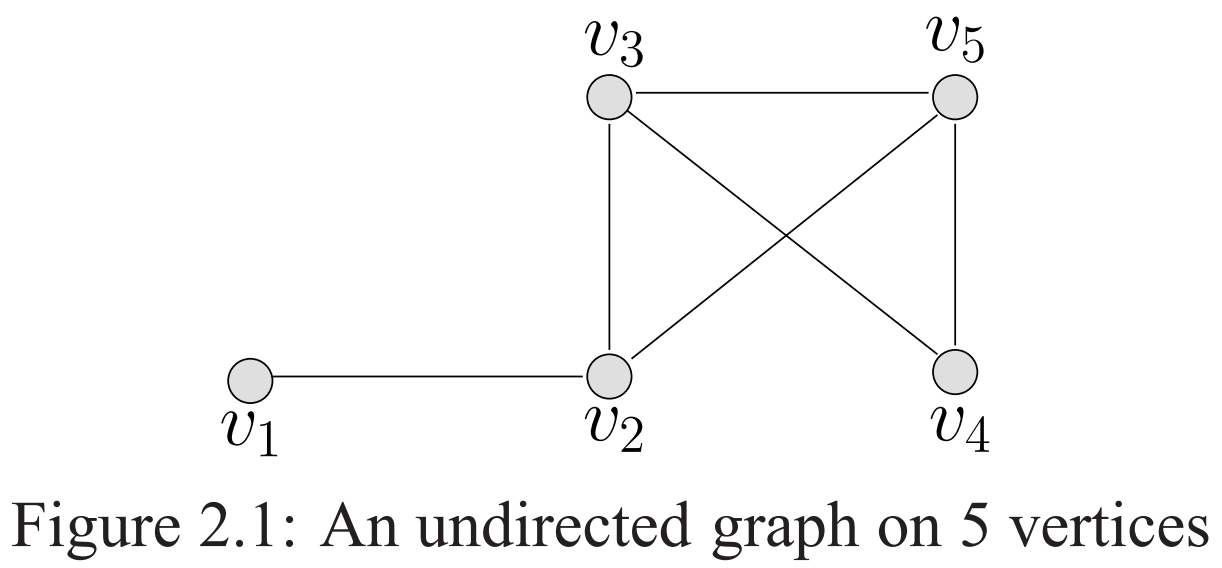
\includegraphics[width=0.8\linewidth]{images/Figure_2_1.png}
    \end{figure}
    \begin{align*}
        V &= \{ v_1, v_2, \dots , v_5 \} \\
        E &= \{ v_1 v_2, v_2 v_3, v_3 v_4, v_3 v_5 , v_2 v_5, v_4 v_5\}
    \end{align*}
    \item The {\color{red}neighborhood} $N(i) \subseteq V$ of the vertex $v_i$ is defined as $N(i) = \{v_j \in V | v_i v_j \in E\}$. $N(i)$ is the set of all vertices that are {\color{red}adjacent} to $v_i$.
    \begin{itemize}
        \item If $v_{\color{red}j} \in N({\color{blue}i})$, then $v_{\color{blue}i} \in N({\color{red}j})$ 
    \end{itemize}
    \item A {\color{blue}path} of length ${\color{red}m}$ in $\mathcal{G}$ is given by a sequence of distinct vertices $v_{i_0}, v_{i_1},\dots , v_{i_{\color{red}m}}$.
\end{itemize}